\documentclass[aspectratio=169,11pt]{beamer}
\usetheme{Madrid}
\usecolortheme{seahorse}
\usepackage[T1]{fontenc}
\usepackage[utf8]{inputenc}
\usepackage{lmodern}
\usepackage{amsmath,amssymb}
\usepackage{tikz}
\usetikzlibrary{arrows.meta,positioning,fit,shapes.geometric}
\usepackage{listings}
\usepackage{booktabs}
\usepackage{graphicx}
\usepackage{xcolor}
\definecolor{codegray}{RGB}{245,245,245}
\definecolor{deepblue}{RGB}{22,74,122}
\setbeamercolor{title}{fg=deepblue}
\setbeamercolor{frametitle}{fg=deepblue}
\setbeamertemplate{navigation symbols}{}
\lstdefinelanguage{Julia}{morekeywords={using,const,function,struct,return,end,for,in,if,else,elseif,begin,let,mutable,where,do,try,catch,finally,global,local,quote,macro,module,import,export},sensitive=true,morecomment=[l]\#,morestring=[b]"}
\lstset{language=Julia,basicstyle=\ttfamily\scriptsize,backgroundcolor=\color{codegray},frame=single,breaklines=true,columns=fullflexible,keepspaces=true}
\title[HPD.jl FCR/FREKI]{HydroPowerDynamics.jl for FCR Studies}
\subtitle{Trollheim AGC branch - FREKI objectives - modular code workflow}
\author{Madhusudhan Pandey}
\date{AGC\_Trollheim / quick\_examples/freki\_objectives}
\begin{document}

\begin{frame}
  \titlepage
  \vfill
  \small Repository focus: \texttt{pandeysudan1/HydroPowerDynamics.jl}, branch \texttt{AGC\_Trollheim}.\\
  Folder focus: \texttt{quick\_examples/freki\_objectives}.
\end{frame}

\begin{frame}{Why this deck exists}
\begin{block}{One practical question}
A Trollheim-like hydropower producer wants FCR revenue, but does not want to start with arbitrary plant tests.
\end{block}
\begin{itemize}
\item Use ordinary plant measurements first.
\item Validate the model block by block.
\item Estimate a conservative FCR candidate.
\item Identify the physical limit and the best operational action.
\item Keep checking model health during operation.
\end{itemize}
\vspace{0.2cm}
\centering
\textbf{Model-based screening capacity $\neq$ formally qualified FCR capacity.}
\end{frame}

\begin{frame}{FREKI objectives mapped to an engineering story}
\begin{enumerate}
\item Validate plant simulation models using real-time/available measurements.
\item Determine how much FCR can be screened using verified models.
\item Identify measures that can increase the FCR candidate.
\item Validate the approach across Francis, Pelton and Kaplan units.
\item Demonstrate online logic with rolling model-health indicators.
\end{enumerate}
\vspace{0.25cm}
\begin{block}{Repository story}
Measurements $\rightarrow$ validated model $\rightarrow$ robust candidate MW $\rightarrow$ limiting mechanism $\rightarrow$ plant-test package.
\end{block}
\end{frame}

\begin{frame}{Trollheim AGC system boundary}
\centering
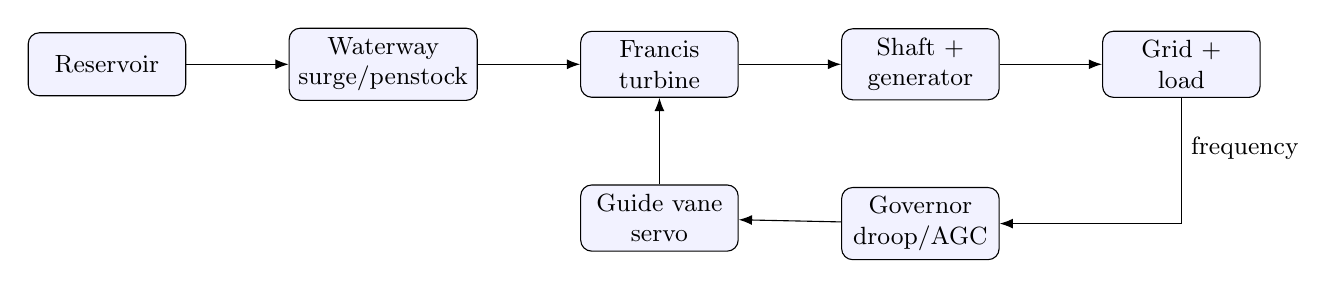
\begin{tikzpicture}[node distance=1.3cm,>=Latex, every node/.style={font=\small}]
\tikzstyle{blk}=[draw, rounded corners, minimum width=2.0cm, minimum height=0.8cm, align=center, fill=blue!5]
\node[blk] (res) {Reservoir};
\node[blk,right=of res] (water) {Waterway\\surge/penstock};
\node[blk,right=of water] (tur) {Francis\\turbine};
\node[blk,right=of tur] (shaft) {Shaft +\\generator};
\node[blk,right=of shaft] (grid) {Grid +\\load};
\node[blk,below=1.1cm of tur] (gate) {Guide vane\\servo};
\node[blk,below=1.1cm of shaft] (gov) {Governor\\droop/AGC};
\draw[->] (res)--(water); \draw[->] (water)--(tur); \draw[->] (tur)--(shaft); \draw[->] (shaft)--(grid);
\draw[->] (grid.south) |- node[pos=0.2,right]{frequency} (gov.east);
\draw[->] (gov)--(gate);
\draw[->] (gate)--(tur);
\end{tikzpicture}
\vspace{0.25cm}
\begin{block}{Control idea}
The grid sees frequency and power. The plant limit is inside the hydraulic, turbine, actuator and shaft chain.
\end{block}
\end{frame}

\begin{frame}[fragile]{Folder-level modular implementation}
\begin{lstlisting}[basicstyle=\ttfamily\tiny]
quick_examples/freki_objectives/
  README.md
  OBJECTIVE_01B_RESULTS.md
  TROLLHEIM_MEASUREMENT_VALIDATION.md
  objective_01_model_validation.jl
  objective_01b_trollheim_measurement_validation.jl
  objective_02_fcr_capacity.jl
  objective_03_increase_fcr.jl
  objective_04_multiturbine_validation.jl
  objective_05_online_monitor.jl
  plots/
  results/
\end{lstlisting}
\vspace{0.2cm}
\begin{block}{Design rule}
Each objective is executable alone, but the story is connected through CSV summaries, plots and the top-level README.
\end{block}
\end{frame}

\begin{frame}{Objective 1 - measurement-supported model trust}
\begin{columns}[T]
\column{0.55\textwidth}
\begin{itemize}
\item Fit the local Trollheim turbine relation using measured pressure, head, discharge, guide-vane, speed and power.
\item Use separate calibration and held-out validation windows.
\item Accept only what the data actually support.
\end{itemize}
\column{0.45\textwidth}
\begin{table}
\small
\begin{tabular}{lr}
\toprule
Metric & Value\\
\midrule
Flow RMSE & 0.07945 m$^3$/s\\
Rel. flow RMSE & 0.219\%\\
Power RMSE & 0.15704 MW\\
Rel. power RMSE & 0.123\%\\
Startup power RMSE & 4.31884 MW\\
\bottomrule
\end{tabular}
\end{table}
\end{columns}
\begin{block}{Decision}
Local turbine map is useful. Full FCR readiness still needs hydraulic and governor dynamic evidence.
\end{block}
\end{frame}

\begin{frame}[fragile]{Objective 2 - robust FCR screening code pattern}
\begin{lstlisting}
struct Scenario
    name::String
    Kq::Float64
    eta_max::Float64
    c_eta::Float64
    H::Float64
    Tg::Float64
end

scenarios = Scenario[
    Scenario("nominal",      KQ_ID,      ETA_ID,      0.25, H0,     0.30),
    Scenario("slow_servo",   KQ_ID,      ETA_ID,      0.25, H0,     0.50),
    Scenario("conservative", 0.985KQ_ID, 0.99ETA_ID,  0.50, 0.98H0, 0.50),
]
\end{lstlisting}
\begin{block}{Pattern}
A scenario set carries uncertainty from model validation into reserve screening.
\end{block}
\end{frame}

\begin{frame}{Objective 2 - FCR capacity result}
\begin{columns}[T]
\column{0.48\textwidth}
\includegraphics[width=\linewidth]{capacity.png}
\column{0.52\textwidth}
\begin{align*}
P_{FCR}^{nominal} &= 10.25\ \mathrm{MW}\\
P_{FCR}^{robust} &= 9.75\ \mathrm{MW}
\end{align*}
\begin{itemize}
\item Plant operates near full gate: $y_0 \approx 0.928$ pu.
\item Conservative scenario reduces capacity by about 0.5 MW.
\item Result is a test-planning number, not a qualification certificate.
\end{itemize}
\end{columns}
\end{frame}

\begin{frame}{Objective 3 - what limits the reserve?}
\begin{block}{Capacity as an engineering function}
\[
P_{FCR}^{max}=F(R,T_g,K_i,\dot{y}_{max},P_0,H,\theta_h,\ldots)
\]
\end{block}
\begin{columns}[T]
\column{0.52\textwidth}
\begin{itemize}
\item Test one intervention at a time.
\item Compare faster servo, guide-vane rate, travel, head and operating point.
\item Best tested intervention: lower operating gate.
\end{itemize}
\column{0.48\textwidth}
\begin{align*}
P_{screen} &= 16.7\ \mathrm{MW}\\
\Delta P &= 6.95\ \mathrm{MW}\\
\mathrm{gain} &= 71.3\% 
\end{align*}
\end{columns}
\end{frame}

\begin{frame}{Objective 4 - same service, different turbine physics}
\centering
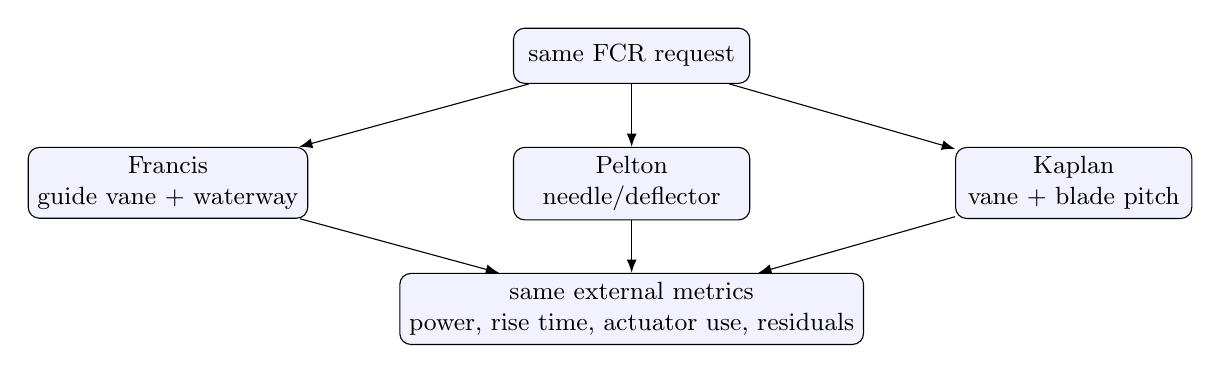
\begin{tikzpicture}[node distance=0.8cm,>=Latex, every node/.style={font=\small}]
\tikzstyle{box}=[draw, rounded corners, align=center, minimum width=3.0cm, minimum height=0.7cm, fill=blue!5]
\node[box] (req) {same FCR request};
\node[box,below left=0.8cm and 2.6cm of req] (fr) {Francis\\guide vane + waterway};
\node[box,below=of req] (pe) {Pelton\\needle/deflector};
\node[box,below right=0.8cm and 2.6cm of req] (ka) {Kaplan\\vane + blade pitch};
\node[box,below=2.4cm of req] (met) {same external metrics\\power, rise time, actuator use, residuals};
\draw[->] (req)--(fr); \draw[->] (req)--(pe); \draw[->] (req)--(ka);
\draw[->] (fr)--(met); \draw[->] (pe)--(met); \draw[->] (ka)--(met);
\end{tikzpicture}
\vspace{0.2cm}
\begin{block}{Rule}
Reuse the qualification workflow; do not reuse Trollheim validation evidence for another turbine.
\end{block}
\end{frame}

\begin{frame}{Objective 5 - online model-health monitor}
\begin{columns}[T]
\column{0.46\textwidth}
\includegraphics[width=\linewidth]{health.png}
\column{0.54\textwidth}
\begin{align*}
r_k &= y_k-\hat{y}_k\\
RMSE_Q,\ RMSE_P &\rightarrow \text{rolling residuals}
\end{align*}
\begin{itemize}
\item 3600 Trollheim samples replayed offline.
\item 60 s rolling window.
\item GREEN fraction: about 88.7\%.
\item FCR number trusted only while health is acceptable.
\end{itemize}
\end{columns}
\end{frame}

\begin{frame}{End-to-end decision chain}
\centering
\begin{tikzpicture}[node distance=0.7cm,>=Latex, every node/.style={font=\scriptsize}]
\tikzstyle{step}=[draw, rounded corners, minimum width=6.8cm, minimum height=0.55cm, align=center, fill=blue!5]
\node[step] (s1) {1. Validate Trollheim model with measurements};
\node[step,below=of s1] (s2) {2. Estimate robust screening capacity: 9.75 MW};
\node[step,below=of s2] (s3) {3. Find active limit: gate headroom};
\node[step,below=of s3] (s4) {4. Test intervention: lower operating point gives 16.7 MW screening};
\node[step,below=of s4] (s5) {5. Monitor residuals: use FCR estimate only when model health is GREEN};
\node[step,below=of s5] (s6) {6. Prepare Statnett/Nordic plant-test evidence package};
\foreach \a/\b in {s1/s2,s2/s3,s3/s4,s4/s5,s5/s6} \draw[->] (\a)--(\b);
\end{tikzpicture}
\end{frame}

\begin{frame}{What goes into the Statnett-facing package?}
\begin{columns}[T]
\column{0.5\textwidth}
\begin{enumerate}
\item Operating point and measurements
\item Validated blocks and AMBER gaps
\item Candidate FCR volume
\item Predicted power/frequency/gate response
\item Active plant constraint
\end{enumerate}
\column{0.5\textwidth}
\begin{enumerate}\setcounter{enumi}{5}
\item Parameter assumptions
\item Test sequence to execute
\item Measurement-vs-model comparison
\item Residual/model-health result
\item Final formal documentation
\end{enumerate}
\end{columns}
\vspace{0.3cm}
\centering
\textbf{The model supports the process before, during and after the physical test.}
\end{frame}

\begin{frame}[fragile]{Run the modular studies}
\begin{lstlisting}[language=bash,basicstyle=\ttfamily\tiny]
julia --project=. -e 'using Pkg; Pkg.instantiate()'
julia --project=. quick_examples/freki_objectives/objective_01b_trollheim_measurement_validation.jl
julia --project=. quick_examples/freki_objectives/objective_02_fcr_capacity.jl
julia --project=. quick_examples/freki_objectives/objective_03_increase_fcr.jl
julia --project=. quick_examples/freki_objectives/objective_04_multiturbine_validation.jl
julia --project=. quick_examples/freki_objectives/objective_05_online_monitor.jl
\end{lstlisting}
\vspace{0.2cm}
\begin{block}{Outputs}
CSV summaries in \texttt{results/}, plots in \texttt{plots/}, narrative evidence in \texttt{README.md}.
\end{block}
\end{frame}

\begin{frame}{Closing: the Trollheim/FREKI message}
\begin{block}{Main technical conclusion}
HydroPowerDynamics.jl can be organized as a modular FCR evidence engine: measurement validation, robust reserve screening, limiting-mechanism diagnosis, turbine-type portability and online model health.
\end{block}
\begin{itemize}
\item Current robust Trollheim screening value: 9.75 MW.
\item Best tested operating action: lower gate/operating point, screening up to 16.7 MW.
\item Formal FCR qualification: not established by the model alone.
\item Next work: stronger hydraulic/governor identification and physical test comparison.
\end{itemize}
\vfill
\small Sources: repository README and objective scripts in \texttt{AGC\_Trollheim/quick\_examples/freki\_objectives}.
\end{frame}

\end{document}
